\documentclass[letter,12pt]{article}
\usepackage[paperheight=27.94cm,paperwidth=21.59cm,bindingoffset=0in,left=3cm,right=2.0cm, top=3.5cm,bottom=2.5cm, headheight=200pt, headsep=1.0\baselineskip]{geometry}
\usepackage{graphicx,lastpage}
\usepackage{upgreek}
\usepackage{censor}
\usepackage[spanish,es-tabla]{babel}
\usepackage{pdfpages}
\usepackage{tabularx}
\usepackage{graphicx}
\usepackage{adjustbox}
\usepackage{xcolor}
\usepackage{colortbl}
\usepackage{rotating}
\usepackage{multirow}
\usepackage[utf8]{inputenc}
\usepackage[T1]{fontenc}
\usepackage{float}
\usepackage{hyperref}

\renewcommand{\tablename}{Tabla}
\usepackage{fancyhdr}
\pagestyle{fancy}

\fancyhead[L]{}
%
\begin{document}
%
   \title{\Huge{Informe Laboratorio 3}}

   \author{\textbf{Sección 6} \\  \\Amaro Figueroa \\ e-mail: amaro.figueroa@mail.udp.cl}

   \date{Octubre de 2026}

   \maketitle

   \tableofcontents

  \newpage


\section{Descripción de actividades}
Su objetivo será auditar la implementación de algoritmos hash aplicados a contraseñas en páginas web desde el lado del cliente, así como evaluar la efectividad de estas medidas contra ataques de tipo Pass the Hash (PtH). Para llevar a cabo esta auditoría, deberá registrarse en un sitio web y crear una cuenta, ingresando una contraseña específica para realizar las pruebas.\par

Al concluir la tarea, es importante que modifique su contraseña por una diferente para garantizar su seguridad.\par

Dado que la cantidad de sitios chilenos que utilizan hash es limitada, se permite realizar esta tarea en cualquier sitio web a nivel mundial. En este sentido, realice las siguientes actividades:


\begin{itemize}
    \item Identificación del algoritmo de hash utilizado para las contraseñas al momento del registro en el sitio.

    \item Identificación del algoritmo de hash utilizado para las contraseñas al momento de iniciar sesión.

    \item Generación del hash de la contraseña desde la consola del navegador, partiendo de la contraseña en texto plano.

    \item Interceptación del tráfico de login utilizando BurpSuite desde su equipo.

    \item Realización de un intento de login, modificando una contraseña incorrecta por el hash obtenido en el punto anterior.

    \item Descripción de las políticas de privacidad o seguridad relacionadas con las contraseñas, incluyendo un enlace a las mismas.

    \item Cuatro conclusiones sobre la seguridad o vulnerabilidad de la implementación observada.




\end{itemize}

\section{Desarrollo de actividades según criterio de rúbrica}

El sitio auditado es el foro \textbf{SA 4x4 Community Forum} (\url{https://www.4x4community.co.za/forum/}), un foro sudafricano de vehículos todoterreno construido sobre \textbf{vBulletin 4.2.5}, que se encuentra detrás del servicio de protección de Cloudflare. Se eligió porque las versiones 3.x y 4.x de vBulletin calculan el hash de la contraseña en el navegador antes de enviarla al servidor. Para las pruebas se creó la cuenta \texttt{Amaro} con la contraseña de laboratorio \texttt{Lab3Cripto2026}, utilizada únicamente para este trabajo.

Todas las capturas del navegador se obtuvieron con las herramientas de desarrollador (DevTools, pestaña \textit{Network} con la opción \textit{Keep log} activa) del navegador Brave, y las de interceptación con Burp Suite Community Edition v2026.8.

\subsection{Identifica el algoritmo de hash utilizado al momento de registrarse en el sitio}

El formulario de registro (\url{https://www.4x4community.co.za/forum/register.php}) contiene, además de los campos visibles de contraseña, dos campos ocultos llamados \texttt{password\_md5} y \texttt{passwordconfirm\_md5} (Figura \ref{fig:reg-fuente}). Su nombre ya indica que el formulario está preparado para enviar un MD5 de la contraseña.

\begin{figure}[H]
    \centering
    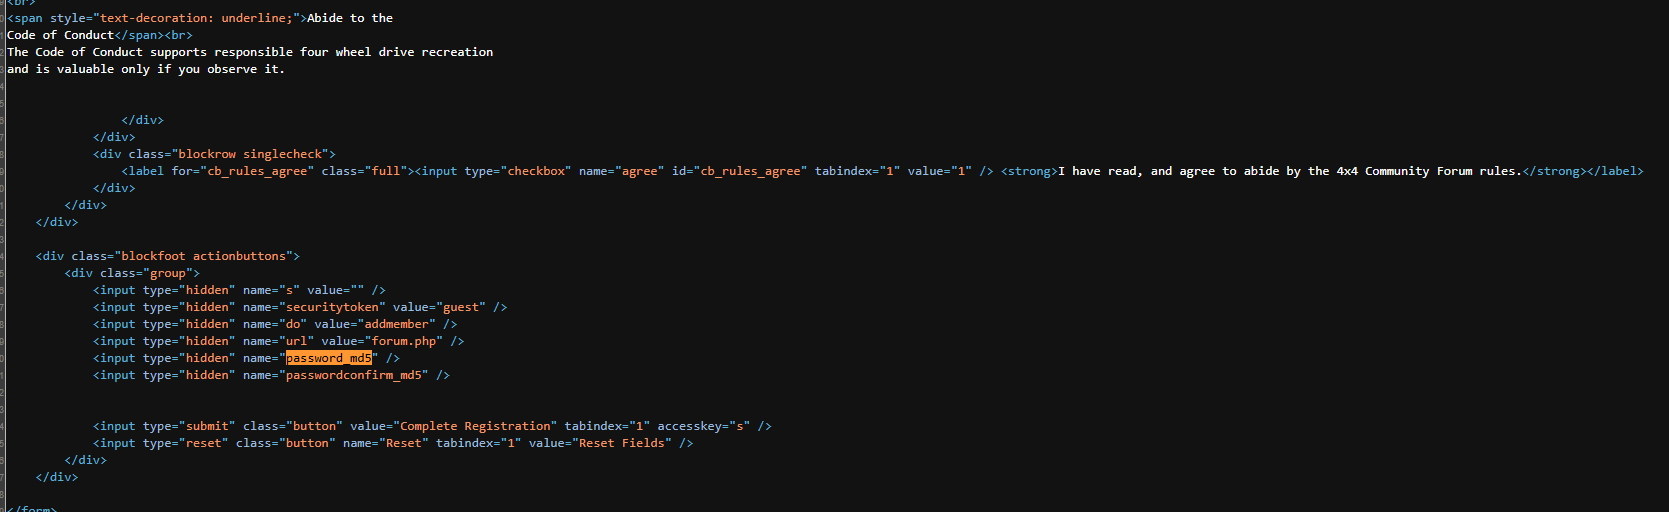
\includegraphics[width=\textwidth]{actividades/registro_codigo_fuente_md5.png}
    \caption{Código fuente del formulario de registro: campos ocultos \texttt{password\_md5} y \texttt{passwordconfirm\_md5}.}
    \label{fig:reg-fuente}
\end{figure}

Al enviar el formulario, el navegador realiza un \texttt{POST} a \texttt{register.php?do=addmember} (Figura \ref{fig:reg-network}). Para documentar el contenido de esta petición se envió el formulario con un código de verificación (captcha) incorrecto a propósito: el navegador calcula y envía el hash de todas formas, pero el servidor rechaza la solicitud, por lo que no se crea una segunda cuenta. En este caso Cloudflare respondió con un código 403 y una verificación anti-bots, lo que no impide ver los datos enviados.

\begin{figure}[H]
    \centering
    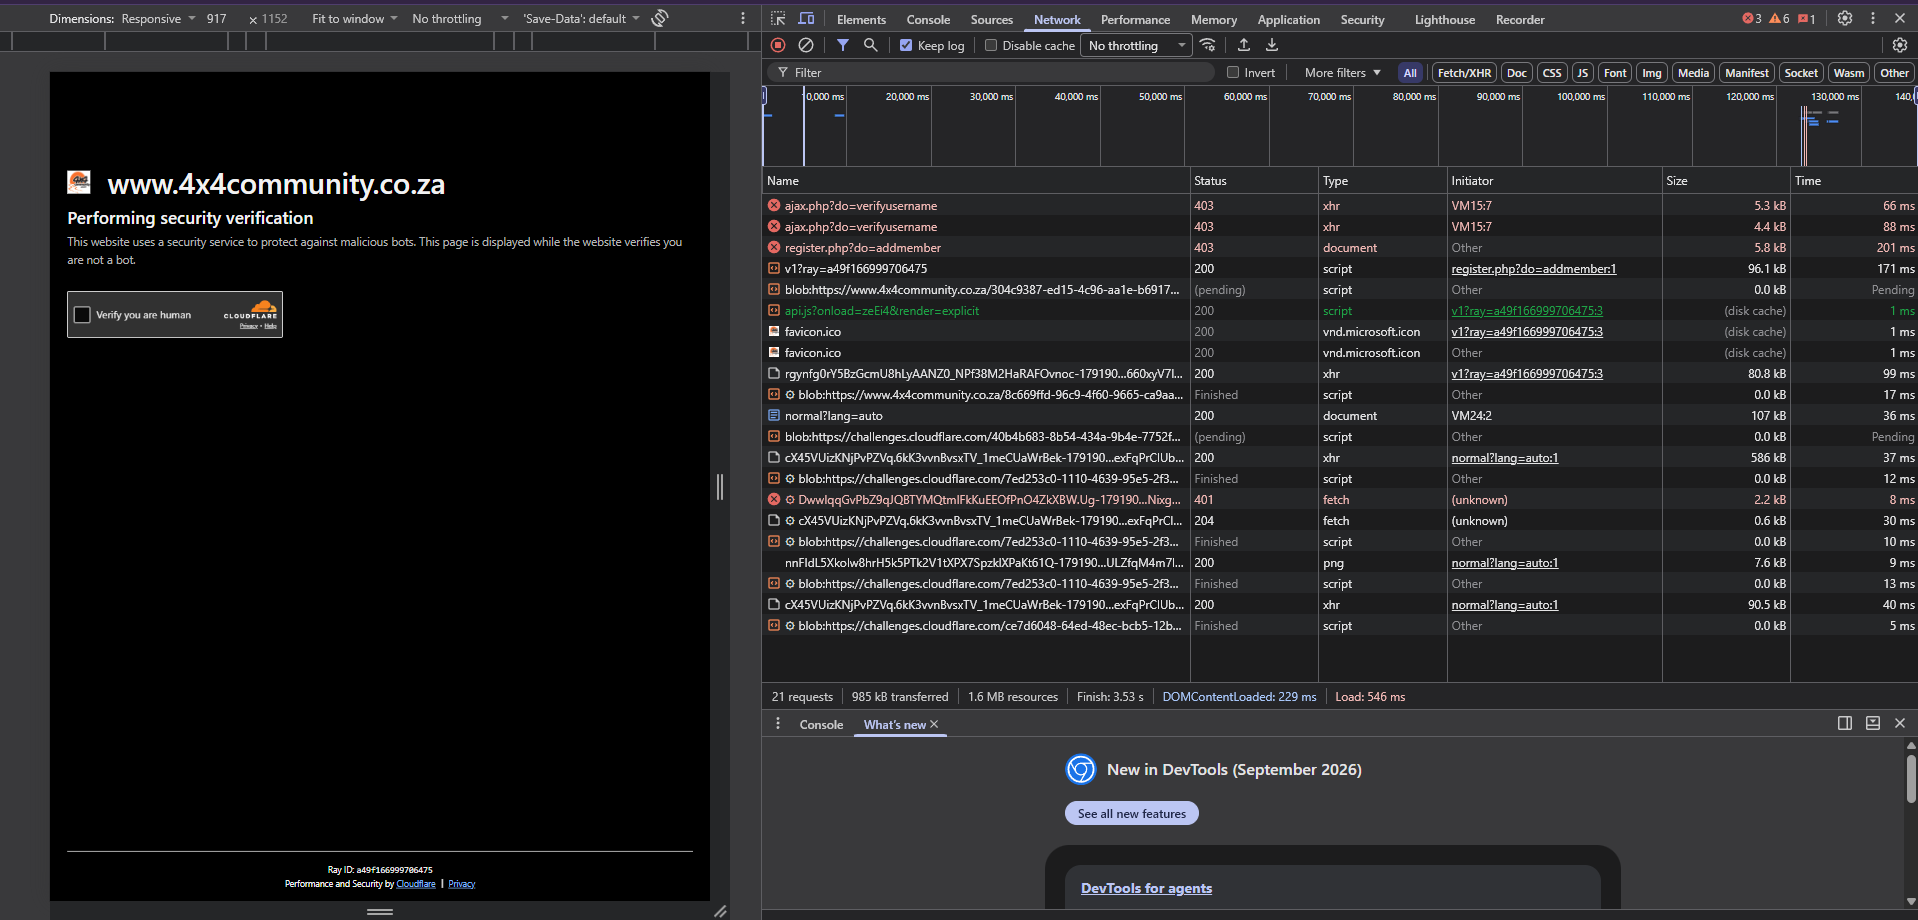
\includegraphics[width=\textwidth]{actividades/registro_post_network.png}
    \caption{Petición \texttt{POST register.php?do=addmember} registrada en la pestaña \textit{Network}.}
    \label{fig:reg-network}
\end{figure}

En el \textit{payload} de la petición (Figuras \ref{fig:reg-payload1} y \ref{fig:reg-payload2}) se observa que:

\begin{itemize}
    \item Los campos \texttt{password} y \texttt{passwordconfirm} viajan \textbf{vacíos}: la contraseña en texto plano nunca sale del navegador.
    \item Los campos \texttt{password\_md5} y \texttt{passwordconfirm\_md5} contienen el mismo valor: \texttt{2a70467ad486f13d79e97b70fc7db373}.
\end{itemize}

\begin{figure}[H]
    \centering
    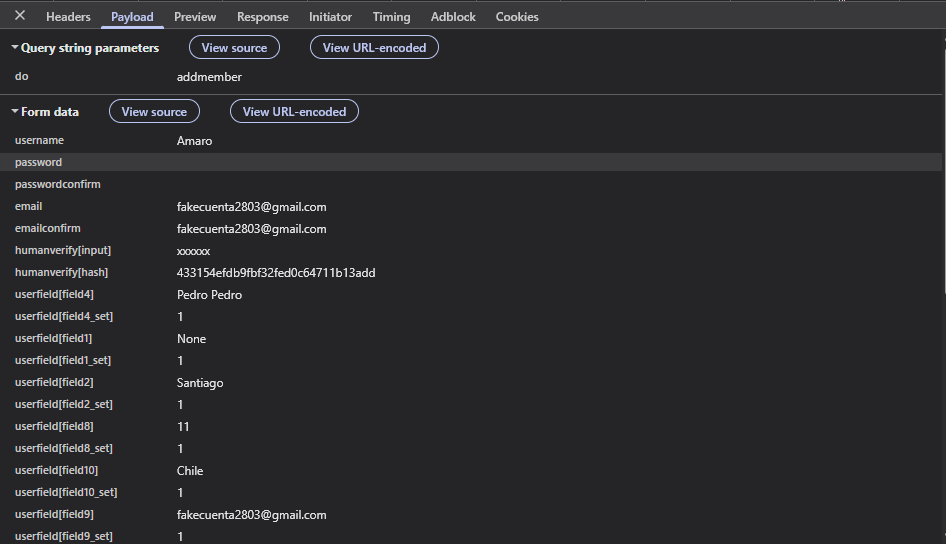
\includegraphics[width=0.85\textwidth]{actividades/registro_payload_1.png}
    \caption{\textit{Payload} del registro (parte 1): los campos \texttt{password} y \texttt{passwordconfirm} van vacíos.}
    \label{fig:reg-payload1}
\end{figure}

\begin{figure}[H]
    \centering
    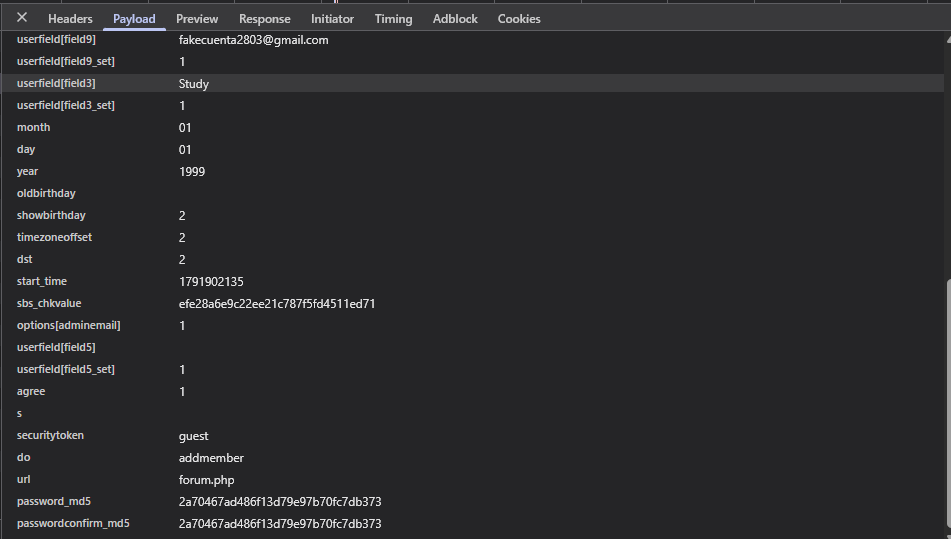
\includegraphics[width=0.85\textwidth]{actividades/registro_payload_2_md5.png}
    \caption{\textit{Payload} del registro (parte 2): \texttt{password\_md5} y \texttt{passwordconfirm\_md5}.}
    \label{fig:reg-payload2}
\end{figure}

El valor tiene 32 caracteres hexadecimales, es decir, 128 bits, que es el largo de salida de MD5 (SHA-1 entrega 160 bits / 40 caracteres y SHA-256 entrega 256 bits / 64 caracteres). Como otros algoritmos también producen 128 bits (por ejemplo MD4 o NTLM), se confirmó calculando el MD5 de \texttt{Lab3Cripto2026}, que da exactamente \texttt{2a70467ad486f13d79e97b70fc7db373} (ver también la sección 2.3). Además, \texttt{password\_md5} y \texttt{passwordconfirm\_md5} son idénticos, lo que muestra que no se agrega sal (un valor aleatorio) en el cliente: es un \textbf{MD5 directo de la contraseña}.

Finalmente, el registro con el captcha correcto se completó y la cuenta quedó a la espera de aprobación de un moderador, aunque con la sesión ya iniciada (Figura \ref{fig:reg-ok}).

\begin{figure}[H]
    \centering
    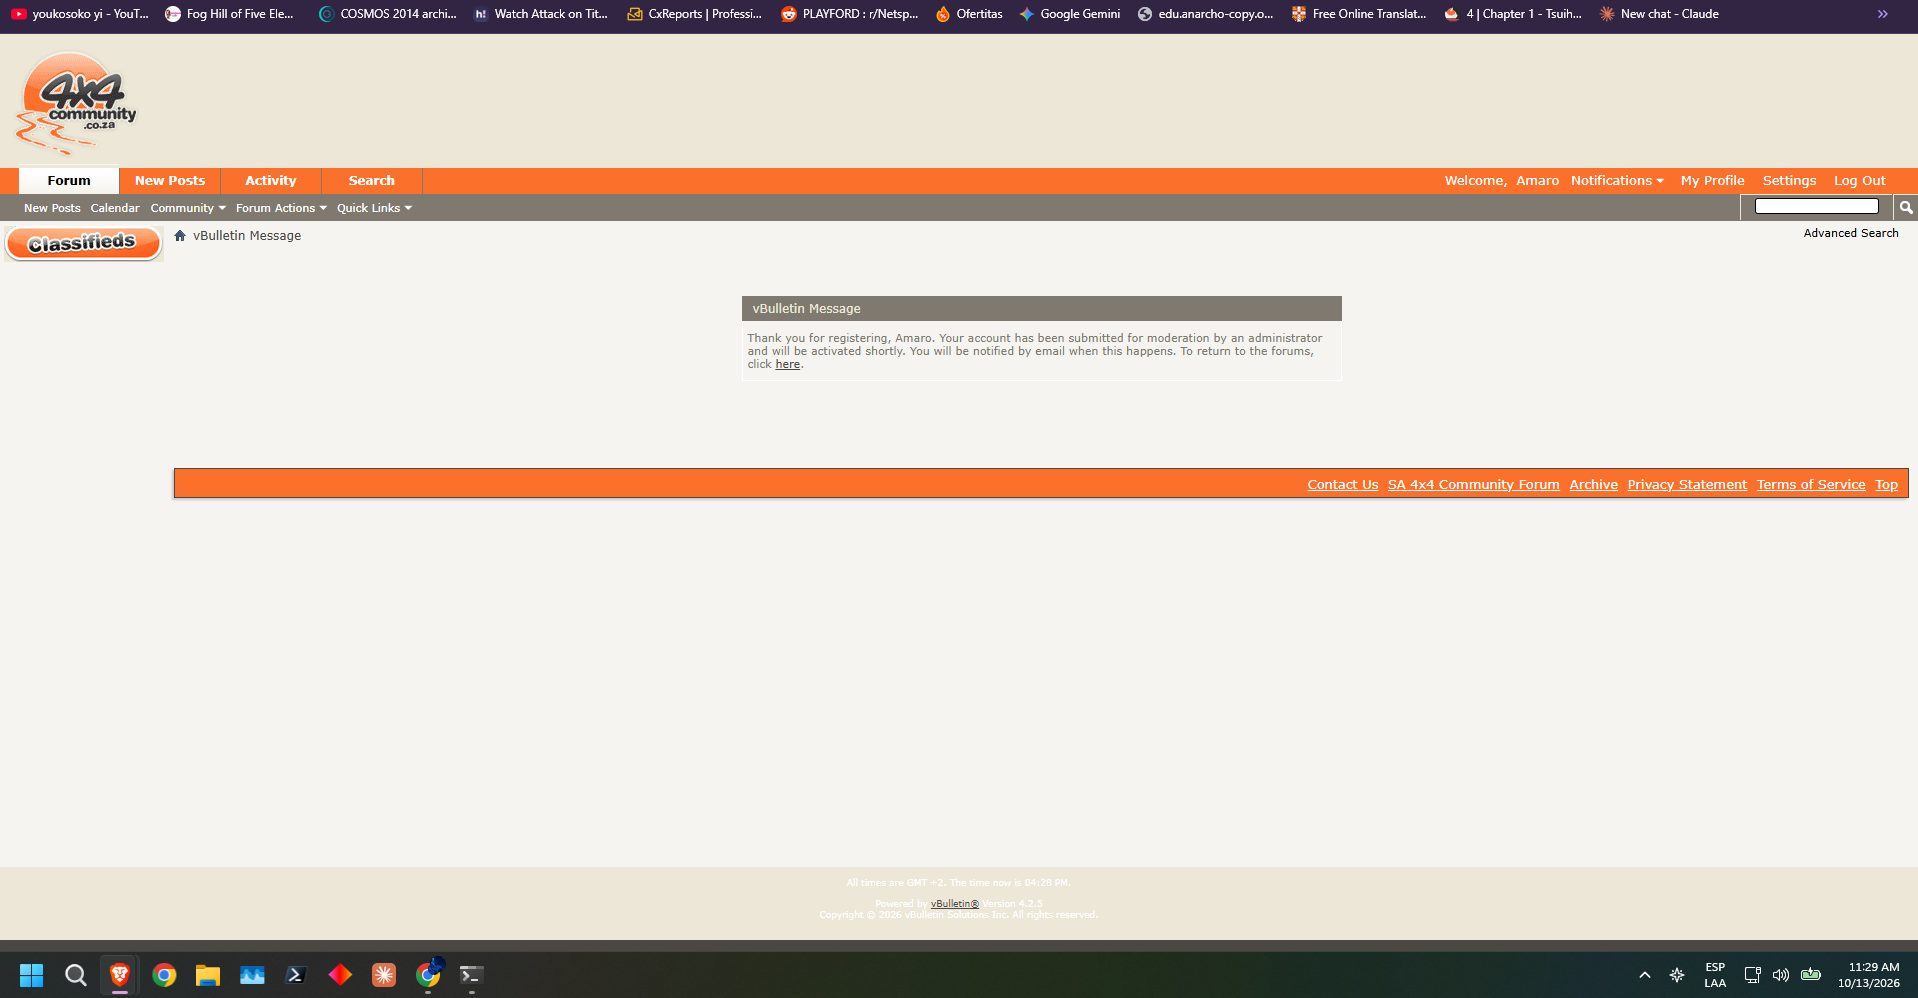
\includegraphics[width=\textwidth]{actividades/registro_completado_moderacion.png}
    \caption{Registro completado: la cuenta \texttt{Amaro} queda pendiente de moderación con la sesión iniciada.}
    \label{fig:reg-ok}
\end{figure}

\textbf{Algoritmo identificado en el registro: MD5, sin sal, calculado en el navegador.}

\subsection{Identifica el algoritmo de hash utilizado al momento de iniciar sesión}

El código fuente de la página con la sesión cerrada (Figura \ref{fig:login-fuente}) muestra:

\begin{itemize}
    \item \textbf{Línea 153}: se carga el archivo \texttt{clientscript/vbulletin\_md5.js}, que contiene la implementación de MD5 en JavaScript.
    \item \textbf{Línea 154}: el formulario de login (\texttt{action="login.php?do=login"}) tiene el evento \texttt{onsubmit="md5hash(vb\_login\_password, vb\_login\_md5password, vb\_login\_md5password\_utf, 0)"}. Antes de enviar, la función \texttt{md5hash} calcula el MD5 de la contraseña, lo guarda en los campos ocultos y vacía el campo de contraseña.
    \item \textbf{Líneas 172 y 173}: los campos ocultos \texttt{vb\_login\_md5password} y \texttt{vb\_login\_md5password\_utf}.
\end{itemize}

\begin{figure}[H]
    \centering
    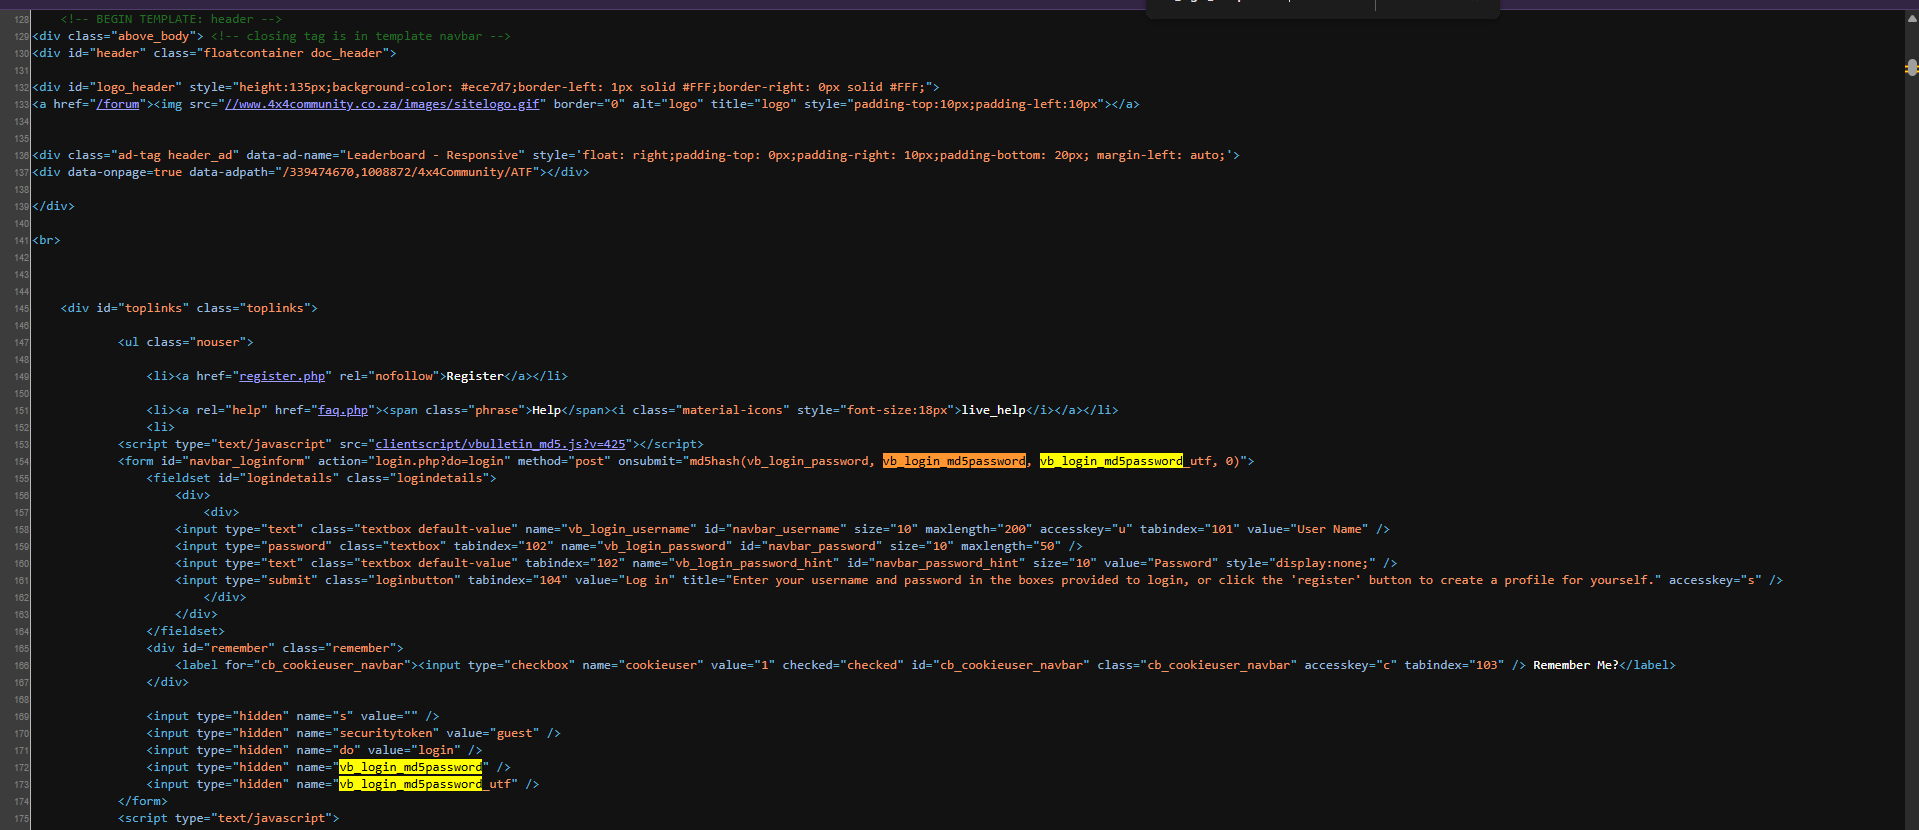
\includegraphics[width=\textwidth]{actividades/login_codigo_fuente_md5.png}
    \caption{Código fuente del formulario de login: carga de \texttt{vbulletin\_md5.js}, llamada a \texttt{md5hash} en \texttt{onsubmit} y campos ocultos.}
    \label{fig:login-fuente}
\end{figure}

Al iniciar sesión con \texttt{Amaro} / \texttt{Lab3Cripto2026}, el navegador envía un \texttt{POST} a \texttt{login.php?do=login} (Figura \ref{fig:login-network}). Cloudflare detuvo esta primera petición con un 403 y una verificación anti-bots; tras superarla, el login se completó.

\begin{figure}[H]
    \centering
    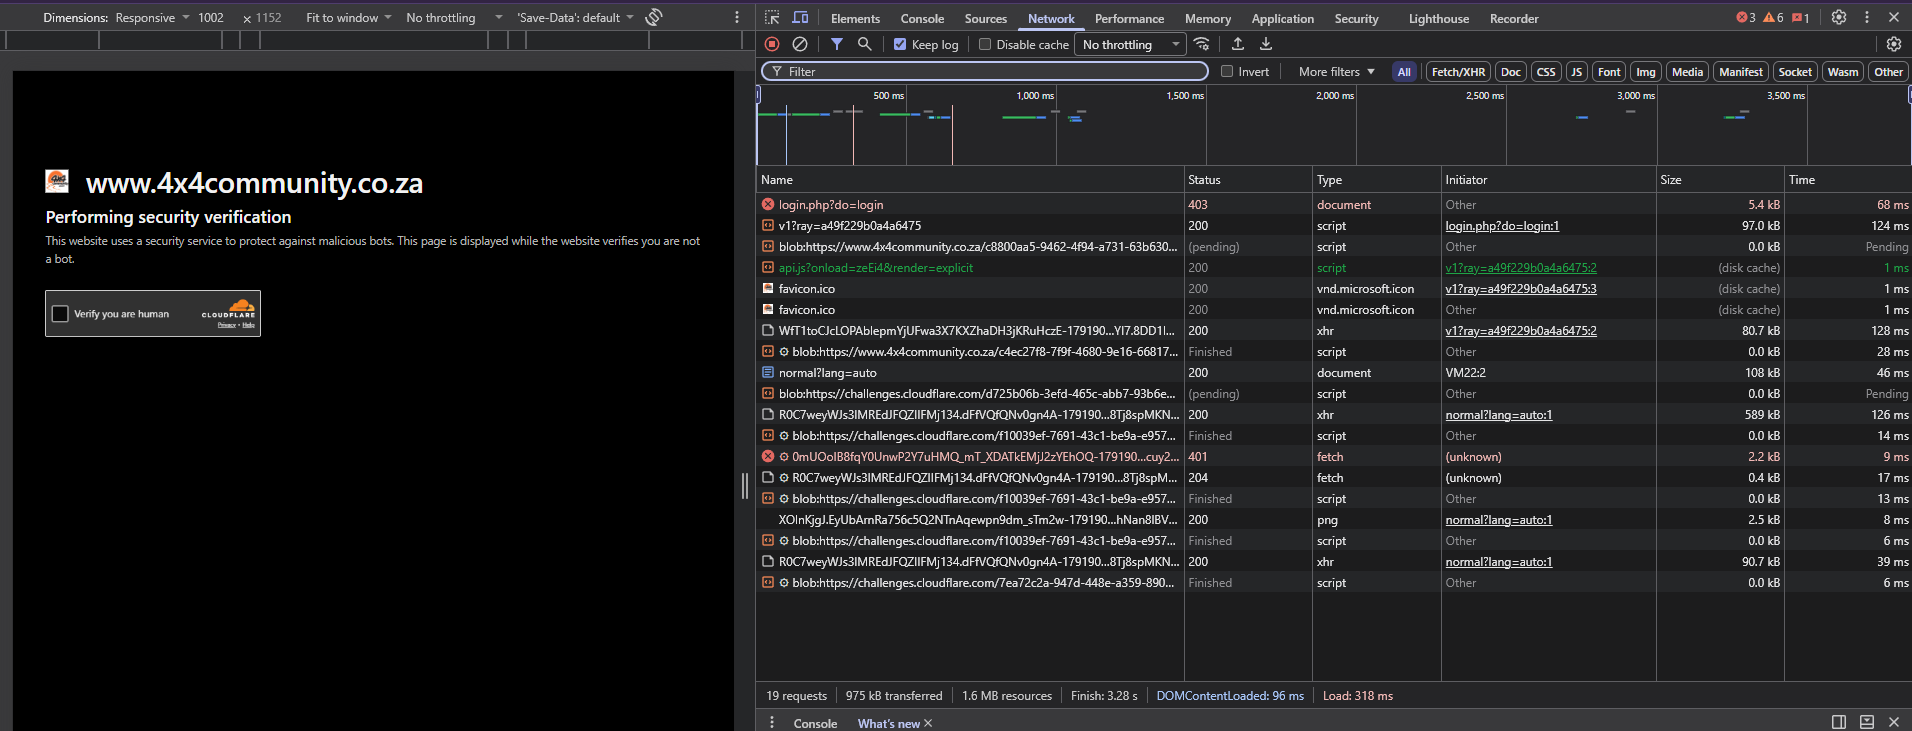
\includegraphics[width=\textwidth]{actividades/login_post_network.png}
    \caption{Petición \texttt{POST login.php?do=login} en la pestaña \textit{Network}.}
    \label{fig:login-network}
\end{figure}

En el \textit{payload} (Figura \ref{fig:login-payload}) el campo \texttt{vb\_login\_password} va vacío, mientras que \texttt{vb\_login\_md5password} y \texttt{vb\_login\_md5password\_utf} contienen \texttt{2a70467ad486f13d79e97b70fc7db373}, \textbf{el mismo valor enviado en el registro}. La variante \texttt{\_utf} existe para contraseñas con caracteres no ASCII; como la contraseña de prueba solo tiene caracteres ASCII, ambos valores coinciden.

\begin{figure}[H]
    \centering
    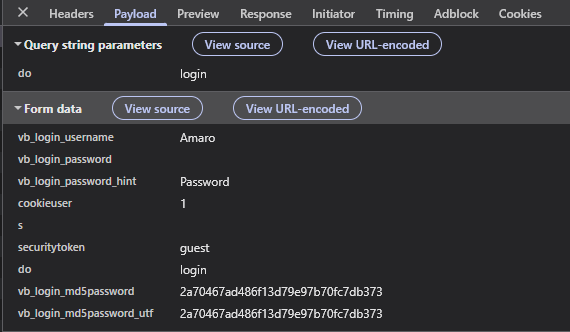
\includegraphics[width=0.7\textwidth]{actividades/login_payload_md5.png}
    \caption{\textit{Payload} del login: \texttt{vb\_login\_password} vacío y el MD5 de la contraseña en los campos ocultos.}
    \label{fig:login-payload}
\end{figure}

Tras superar la verificación de Cloudflare, el servidor aceptó el hash y la página muestra la sesión iniciada como \texttt{Amaro} (Figura \ref{fig:login-ok}).

\begin{figure}[H]
    \centering
    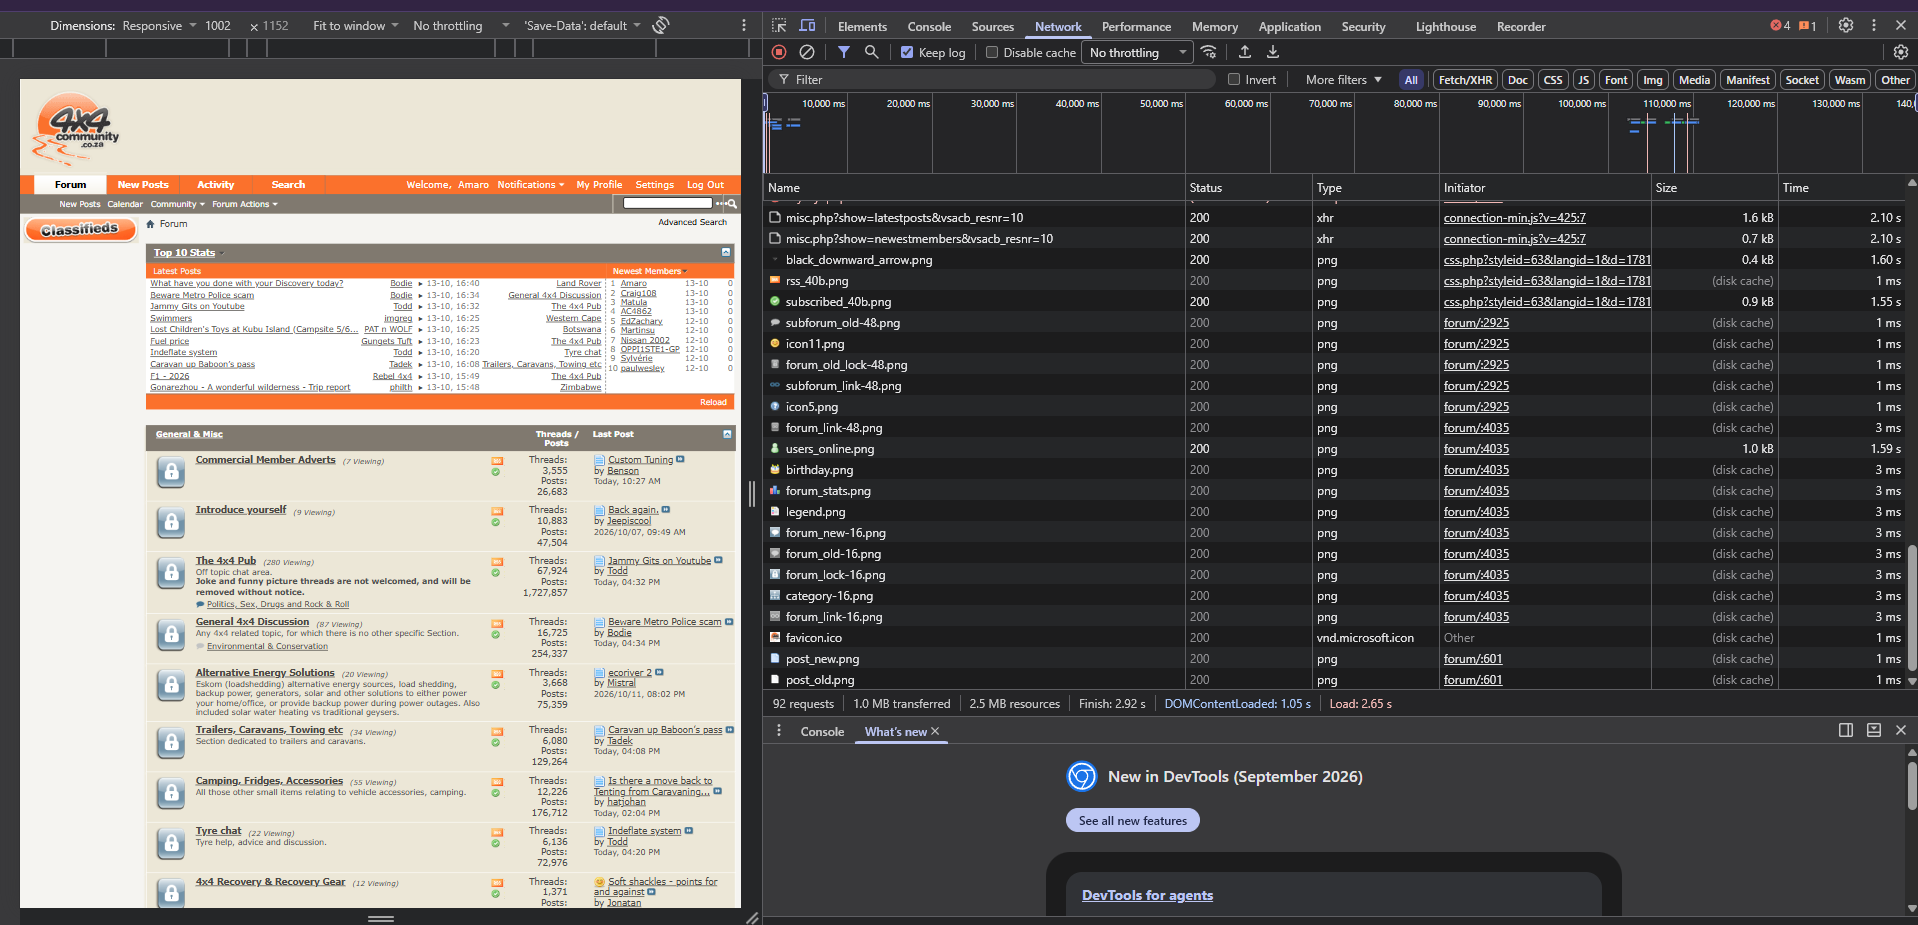
\includegraphics[width=\textwidth]{actividades/login_exitoso.png}
    \caption{Login exitoso: la página muestra ``Welcome, Amaro''.}
    \label{fig:login-ok}
\end{figure}

\textbf{Algoritmo identificado en el login: MD5, sin sal y sin ningún valor aleatorio por sesión.} El valor enviado es siempre el mismo en cada inicio de sesión y coincide con el del registro, por lo que el servidor recibe únicamente el hash y lo trata como si fuera la contraseña. Esta observación es la base del ataque de la sección 2.5.

\subsection{Genera el hash de la contraseña desde la consola del navegador}

El archivo \texttt{vbulletin\_md5.js} define la función global \texttt{hex\_md5}, que se puede llamar desde la consola de DevTools. Este archivo solo se carga cuando la sesión está cerrada (junto al formulario de login), por lo que la prueba se hizo después de cerrar sesión; con la sesión iniciada, la consola responde \texttt{hex\_md5 is not defined}.

Se ejecutaron dos instrucciones (Figura \ref{fig:consola}):

\begin{itemize}
    \item \texttt{hex\_md5("Lab3Cripto2026")} devuelve \texttt{'2a70467ad486f13d79e97b70fc7db373'}, idéntico al valor enviado en el registro y en el login.
    \item \texttt{hex\_md5.toString()} muestra el cuerpo de la función, \texttt{binl2hex(core\_md5(str2binl(A), A.length*chrsz))}, que corresponde a la implementación clásica de MD5 en JavaScript (Paul Johnston) incluida en vBulletin.
\end{itemize}

\begin{figure}[H]
    \centering
    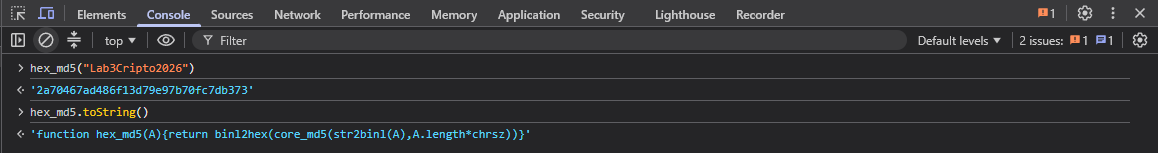
\includegraphics[width=\textwidth]{actividades/consola_hex_md5.png}
    \caption{Generación del hash desde la consola del navegador con la función \texttt{hex\_md5} del propio sitio.}
    \label{fig:consola}
\end{figure}

Esto confirma que cualquier persona que conozca la contraseña puede generar el valor exacto que el servidor espera, usando el mismo código que entrega el sitio.

\subsection{Intercepta el tráfico login con BurpSuite}

Se utilizó el navegador integrado de Burp Suite (\textit{Proxy} $\rightarrow$ \textit{Intercept} $\rightarrow$ \textit{Open browser}), que ya envía todo su tráfico a través del proxy de Burp. Como la página del foro carga una gran cantidad de anuncios que llenaban la cola de intercepción, se agregó una regla en \textit{Proxy settings} $\rightarrow$ \textit{Request interception rules} para interceptar solo las peticiones cuyo dominio coincide con \texttt{4x4community\textbackslash.co\textbackslash.za}.

Con la intercepción activa se intentó iniciar sesión con el usuario \texttt{Amaro} y una contraseña \textbf{incorrecta}: \texttt{ClaveIncorrecta}. Burp detuvo la petición \texttt{POST /forum/login.php?do=login} antes de que llegara al servidor (Figura \ref{fig:burp-cola}).

\begin{figure}[H]
    \centering
    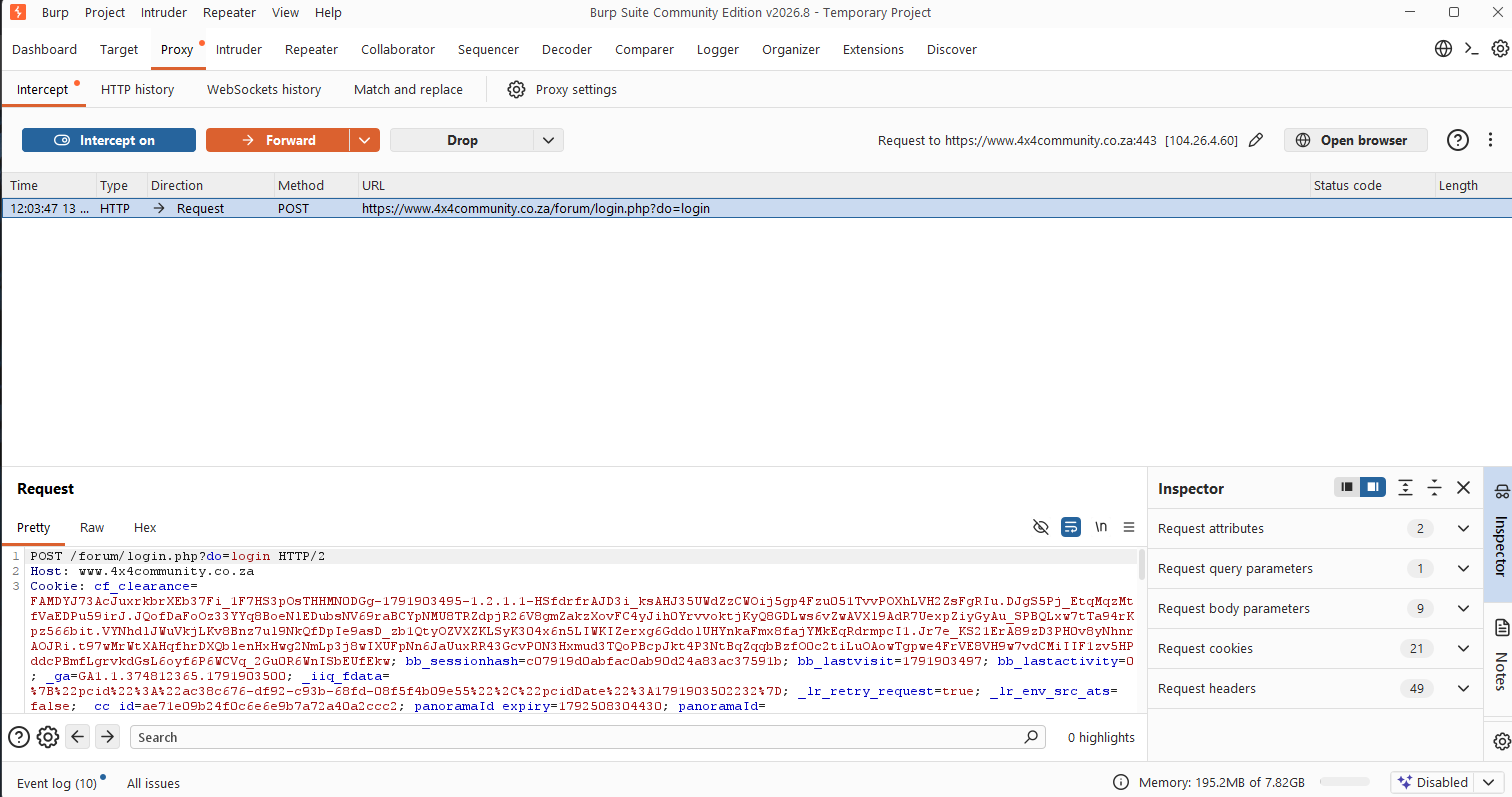
\includegraphics[width=\textwidth]{actividades/burp_intercept_login_cola.png}
    \caption{Burp Suite intercepta la petición \texttt{POST /forum/login.php?do=login}.}
    \label{fig:burp-cola}
\end{figure}

El cuerpo de la petición (Figuras \ref{fig:burp-body} y \ref{fig:burp-inspector}) contiene \texttt{vb\_login\_password} vacío y \texttt{vb\_login\_md5password = 574996f324237db99ec3c55b4a506235}, que es el MD5 de \texttt{ClaveIncorrecta}. Burp ve el tráfico en claro porque actúa como intermediario de la conexión TLS con su propio certificado, en el que confía su navegador integrado.

\begin{figure}[H]
    \centering
    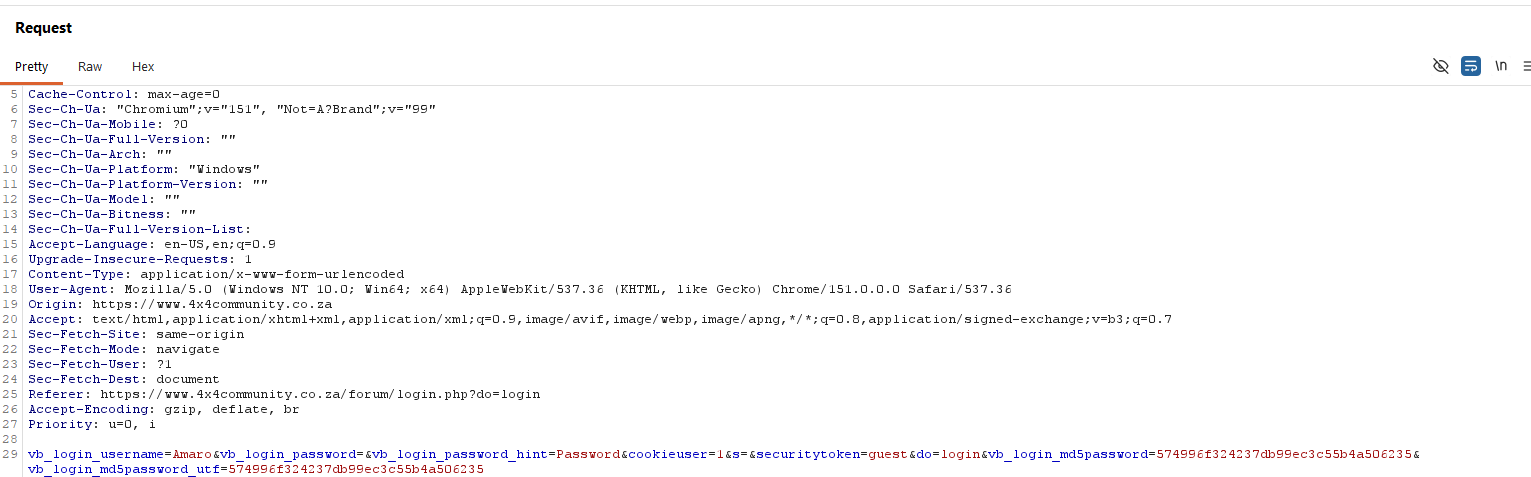
\includegraphics[width=\textwidth]{actividades/burp_intercept_body.png}
    \caption{Cuerpo de la petición interceptada (línea 29): MD5 de la contraseña incorrecta.}
    \label{fig:burp-body}
\end{figure}

\begin{figure}[H]
    \centering
    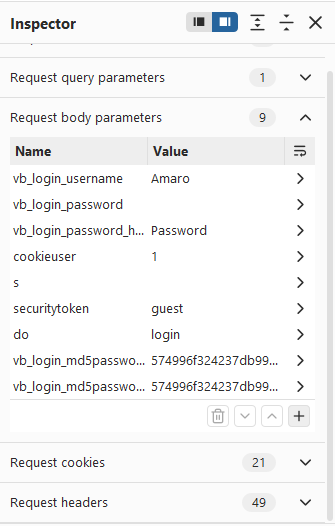
\includegraphics[width=0.5\textwidth]{actividades/burp_intercept_inspector.png}
    \caption{Parámetros del cuerpo de la petición en el panel \textit{Inspector} de Burp.}
    \label{fig:burp-inspector}
\end{figure}

\subsection{Realiza el intento de login}

Sobre la misma petición interceptada se reemplazaron los valores de \texttt{vb\_login\_md5password} y \texttt{vb\_login\_md5password\_utf} por el hash de la contraseña real obtenido en las secciones anteriores, \texttt{2a70467ad486f13d79e97b70fc7db373}, sin modificar nada más (Figura \ref{fig:pth-mod}). Luego se reenvió la petición con \textit{Forward}.

\begin{figure}[H]
    \centering
    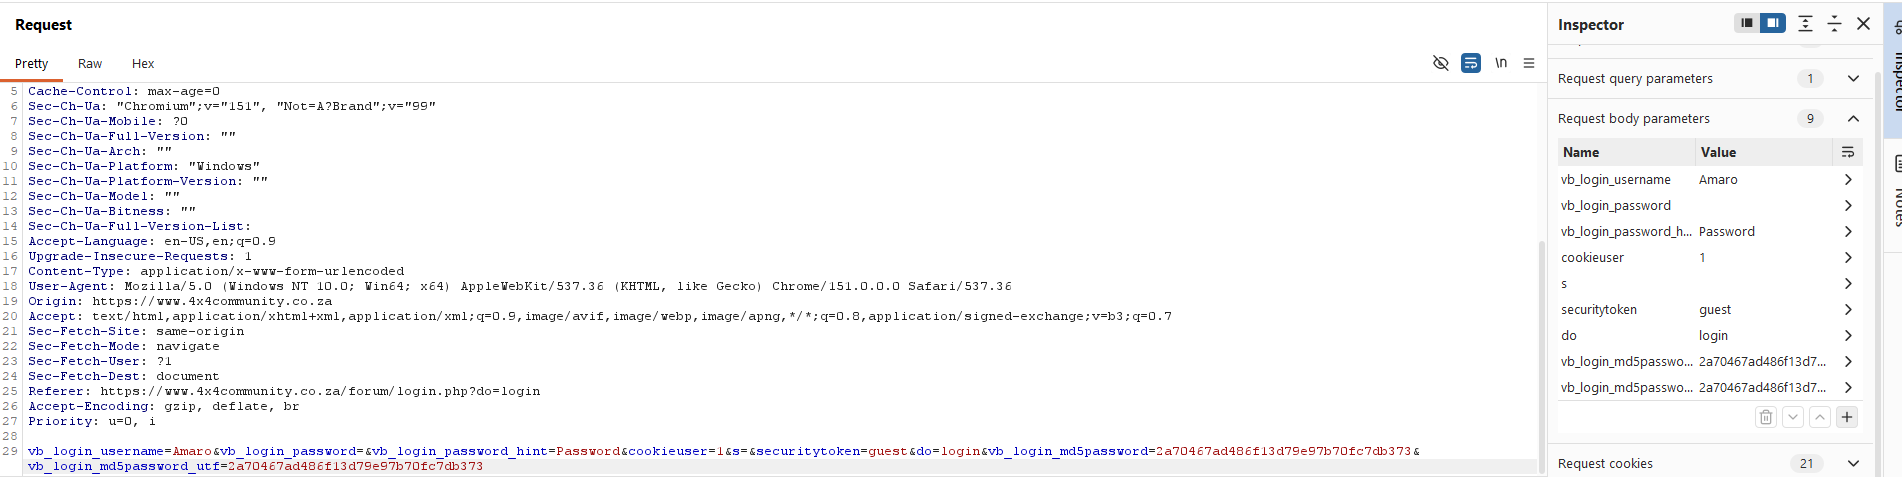
\includegraphics[width=\textwidth]{actividades/burp_pth_modificado.png}
    \caption{Petición modificada: el hash de la contraseña incorrecta se reemplaza por el hash de la contraseña real.}
    \label{fig:pth-mod}
\end{figure}

El servidor aceptó la petición. En el historial de Burp (\textit{Proxy} $\rightarrow$ \textit{HTTP history}, petición 1366 marcada como \textit{Edited}) se conservan ambas versiones: la original, con el hash de \texttt{ClaveIncorrecta} (Figura \ref{fig:pth-orig}), y la editada, con el hash real (Figura \ref{fig:pth-edit}). La respuesta del servidor contiene el mensaje \textbf{``Thank you for logging in, Amaro.''}

\begin{figure}[H]
    \centering
    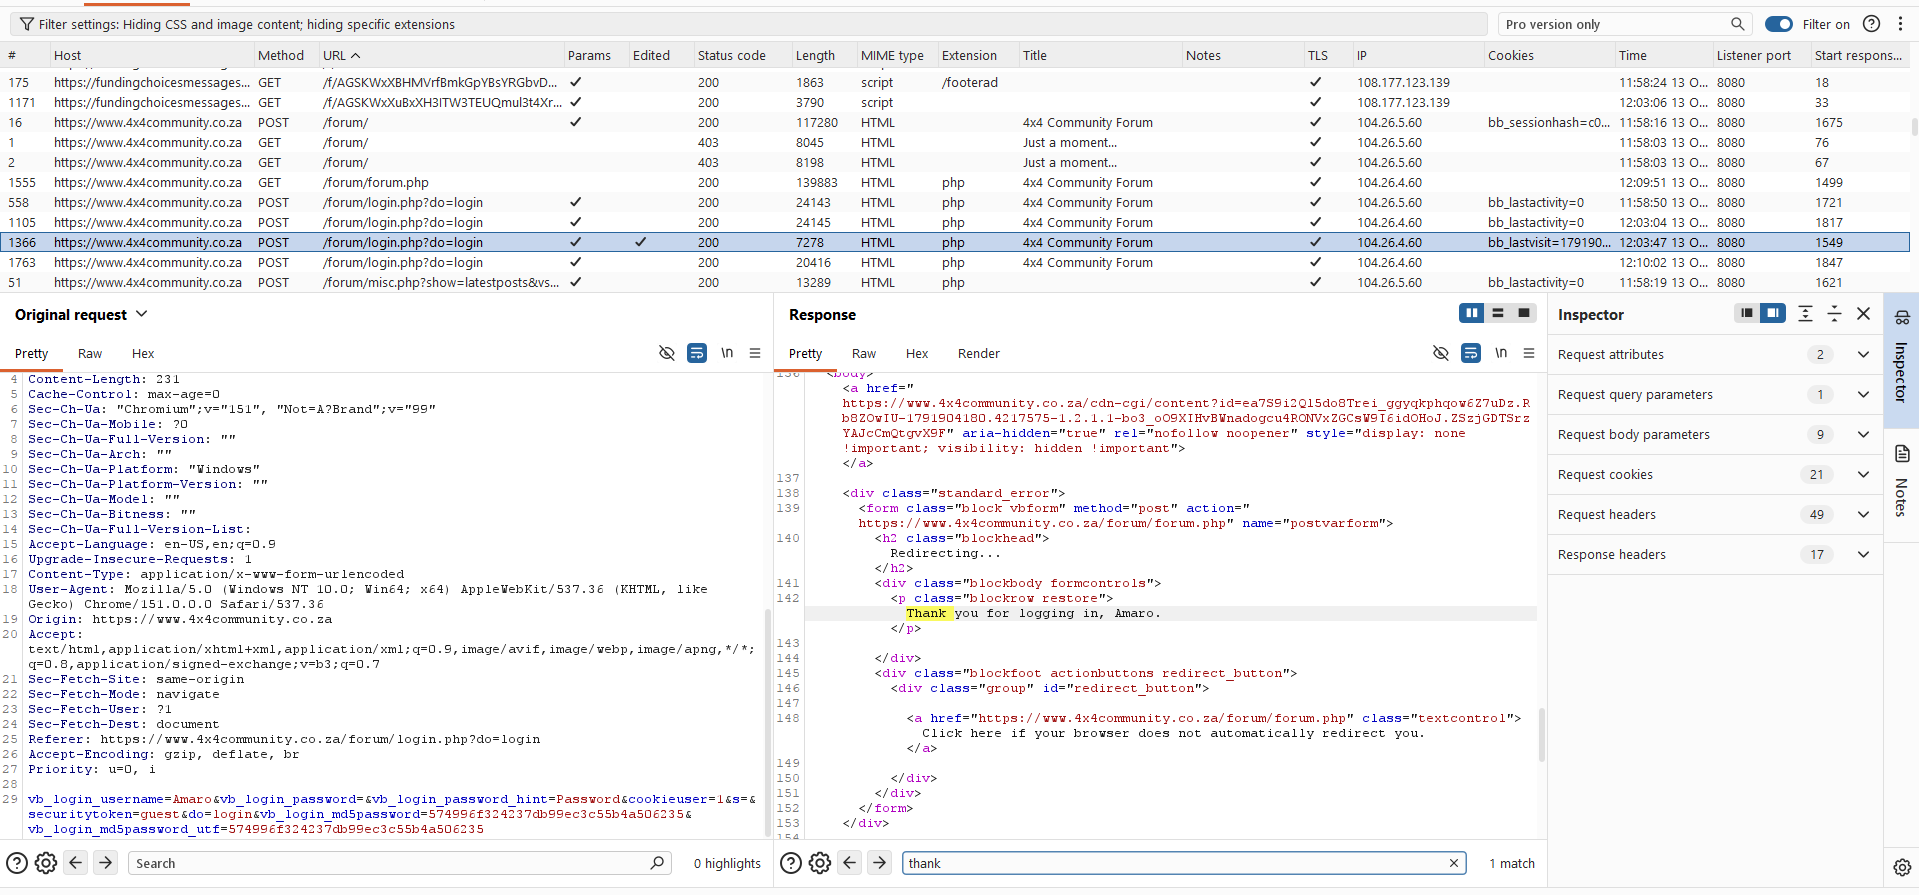
\includegraphics[width=\textwidth]{actividades/burp_history_original_thankyou.png}
    \caption{Historial de Burp: petición original (hash de \texttt{ClaveIncorrecta}) y respuesta del servidor.}
    \label{fig:pth-orig}
\end{figure}

\begin{figure}[H]
    \centering
    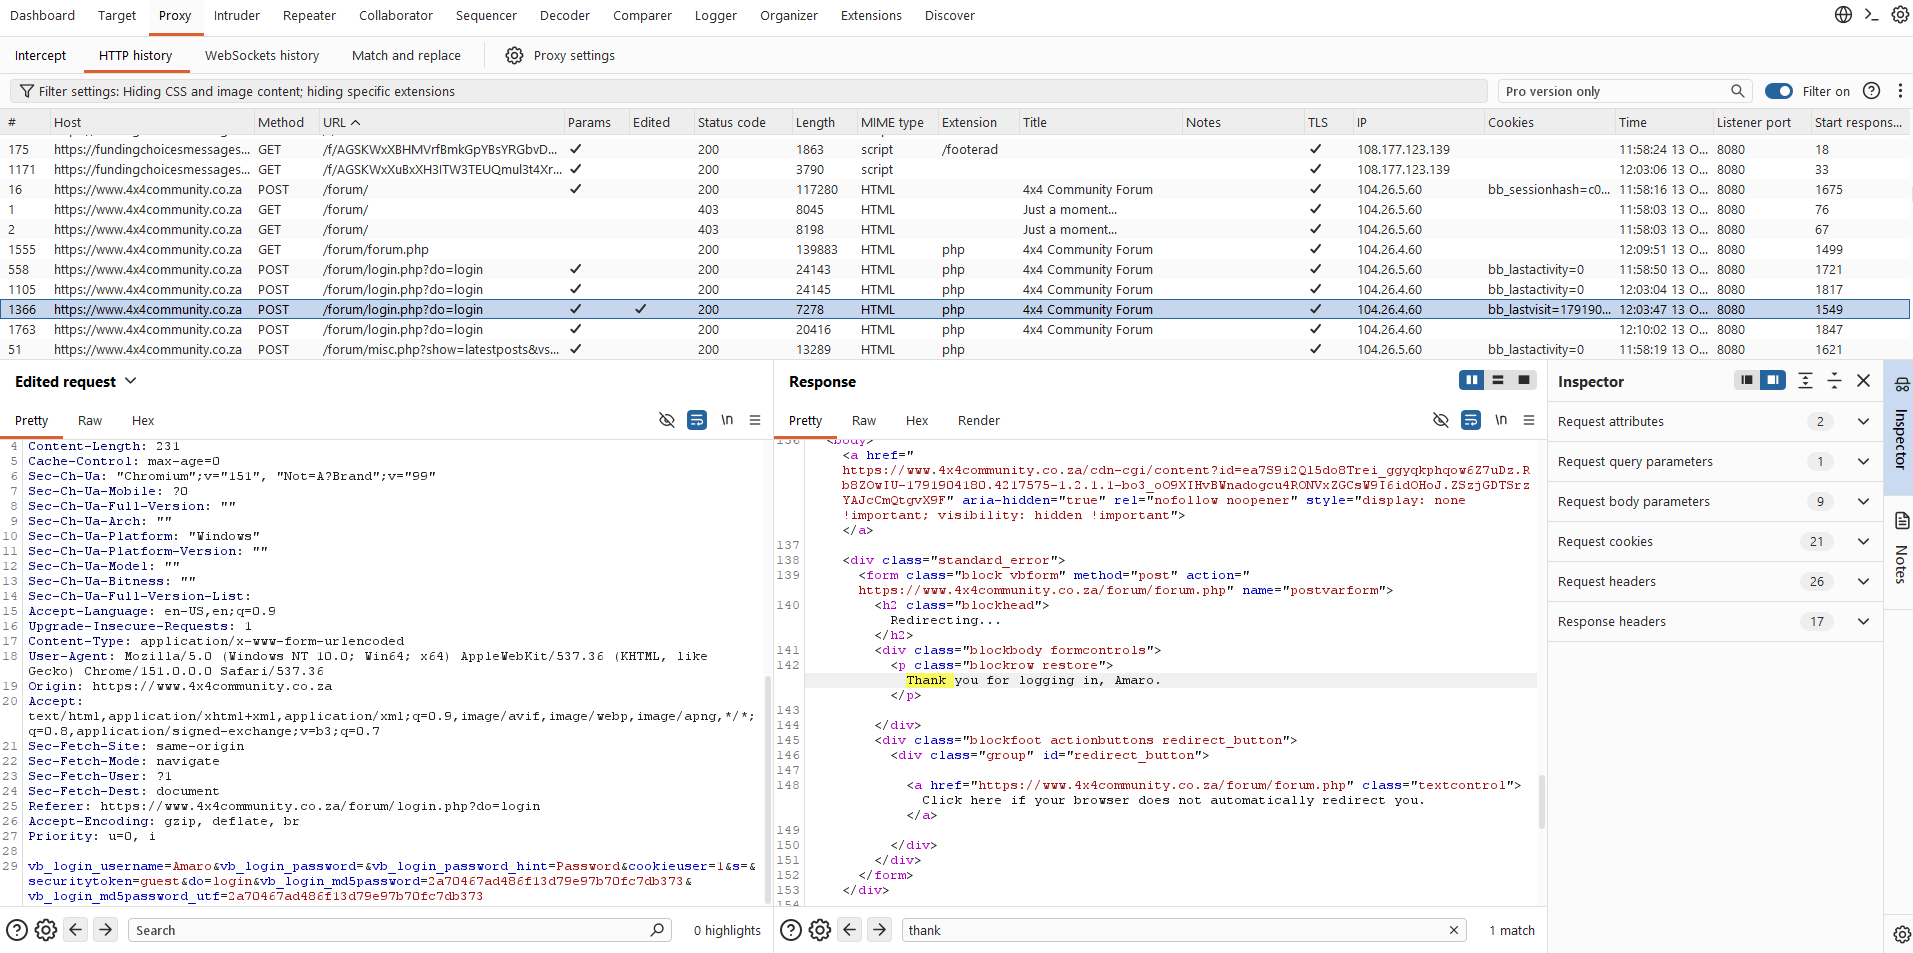
\includegraphics[width=\textwidth]{actividades/burp_history_editado_thankyou.png}
    \caption{Historial de Burp: petición editada (hash real) y respuesta ``Thank you for logging in, Amaro.''}
    \label{fig:pth-edit}
\end{figure}

El navegador fue redirigido a la página principal con la sesión iniciada como \texttt{Amaro} (Figura \ref{fig:pth-ok}).

\begin{figure}[H]
    \centering
    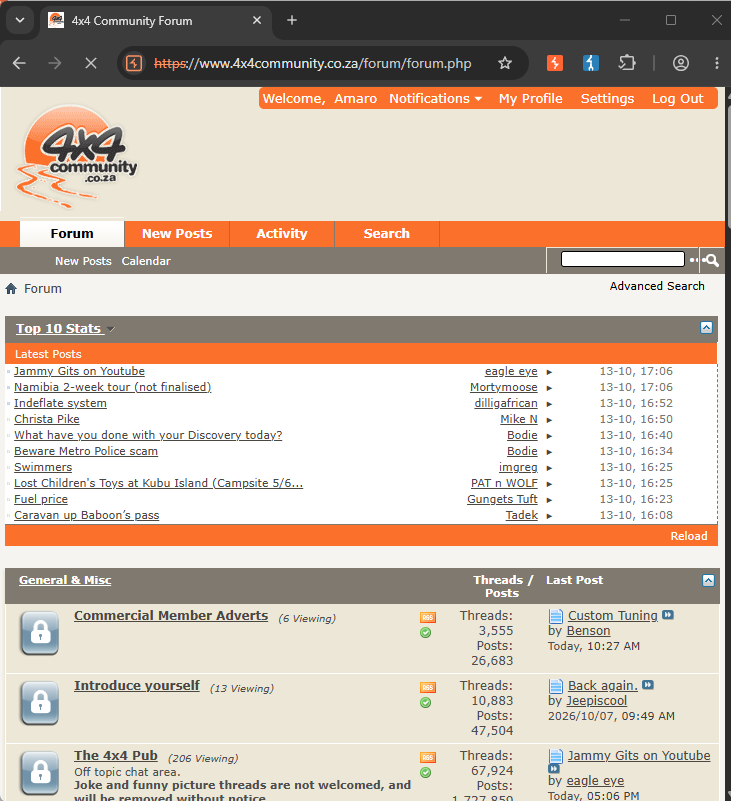
\includegraphics[width=0.7\textwidth]{actividades/burp_pth_login_exitoso.png}
    \caption{Sesión iniciada como \texttt{Amaro} tras el ataque Pass the Hash.}
    \label{fig:pth-ok}
\end{figure}

El ataque \textbf{Pass the Hash fue exitoso}: se inició sesión escribiendo una contraseña incorrecta y entregando solo el hash de la correcta. Esto demuestra que, para este sitio, el hash MD5 \textbf{equivale a la contraseña}: quien obtenga ese valor (por ejemplo, interceptando tráfico, desde un registro del servidor o desde una filtración) puede autenticarse sin conocer ni descifrar la contraseña original.

\subsection{Identifica las políticas de privacidad o seguridad}

El foro publica su política de privacidad en \url{https://www.4x4community.co.za/forum/privacy.php} (Figura \ref{fig:privacidad}), enlazada desde el pie de página como ``Privacy Statement''.

\begin{figure}[H]
    \centering
    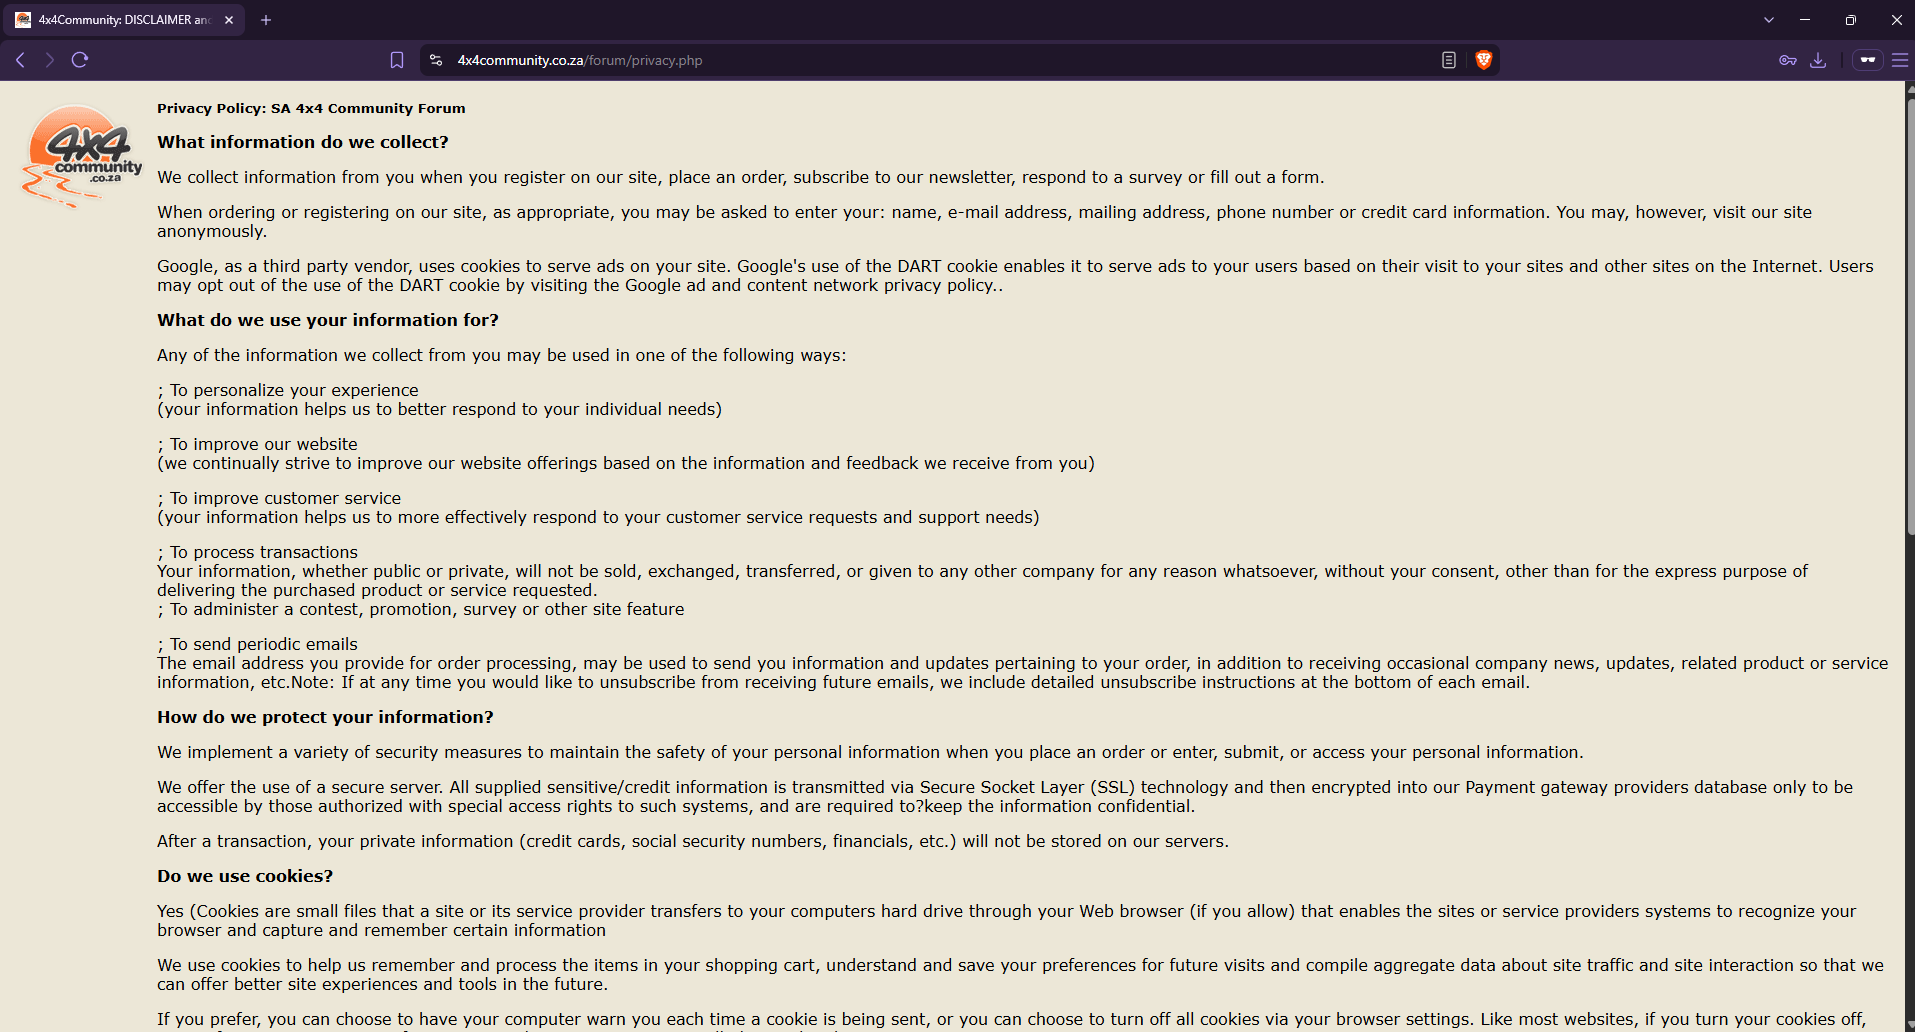
\includegraphics[width=\textwidth]{actividades/politica_privacidad.png}
    \caption{Política de privacidad del foro.}
    \label{fig:privacidad}
\end{figure}

Los puntos principales de la política son:

\begin{itemize}
    \item \textbf{Datos recolectados}: nombre, correo, dirección, teléfono e incluso tarjeta de crédito, al registrarse, comprar, suscribirse o responder encuestas. Google usa la cookie DART y la empresa Adnimation cookies propias y de terceros para publicidad.
    \item \textbf{Protección}: declara implementar ``una variedad de medidas de seguridad'', ofrecer un ``servidor seguro'' y transmitir la información sensible o de pago mediante SSL, y no almacenar datos de tarjetas después de una transacción.
    \item \textbf{Divulgación}: no vende ni transfiere datos personales a terceros, salvo a proveedores de confianza o por requerimiento legal; la información no identificable sí puede compartirse con fines de marketing.
    \item \textbf{Derechos del usuario}: puede editar su información desde ``Edit Profile''; los cambios en la política se publican en la misma página.
\end{itemize}

Adicionalmente, las reglas del foro aceptadas al registrarse exigen datos reales en el perfil (no se permiten cuentas anónimas), prohíben múltiples cuentas por persona e indican que el contenido publicado permanece en el sitio aunque se elimine la cuenta.

\textbf{En relación con las contraseñas, la política no dice nada}: no menciona cómo se transmiten ni cómo se almacenan, qué algoritmo de hash se usa, si se exige una contraseña mínima, si existe autenticación de dos factores ni qué ocurre ante una filtración. Además, es una plantilla genérica de comercio electrónico (habla de carritos de compra, pedidos, tarjetas y números de seguridad social) que no corresponde a un foro. La única medida concreta es el uso de SSL/TLS, que es justamente lo único que protege hoy al hash MD5 en tránsito.

\textbf{Cambio de contraseña al finalizar y manejo de la contraseña al restablecerla.} Como pide el enunciado, al terminar las pruebas se cambió la contraseña de la cuenta, ya que \texttt{Lab3Cripto2026} y su hash quedan expuestos en este informe y, como se demostró, el hash basta para iniciar sesión.

El formulario de cambio de contraseña (\textit{Settings} $\rightarrow$ \textit{Edit Email \& Password}) sigue el mismo esquema que el registro y el login: los campos \texttt{currentpassword}, \texttt{newpassword} y \texttt{newpasswordconfirm} viajan vacíos y solo se envían sus versiones \texttt{\_md5} (Figura \ref{fig:cambio-payload}). El valor de \texttt{currentpassword\_md5} es nuevamente \texttt{2a70467ad486f13d79e97b70fc7db373}. La contraseña nueva de esta captura fue solo temporal.

\begin{figure}[H]
    \centering
    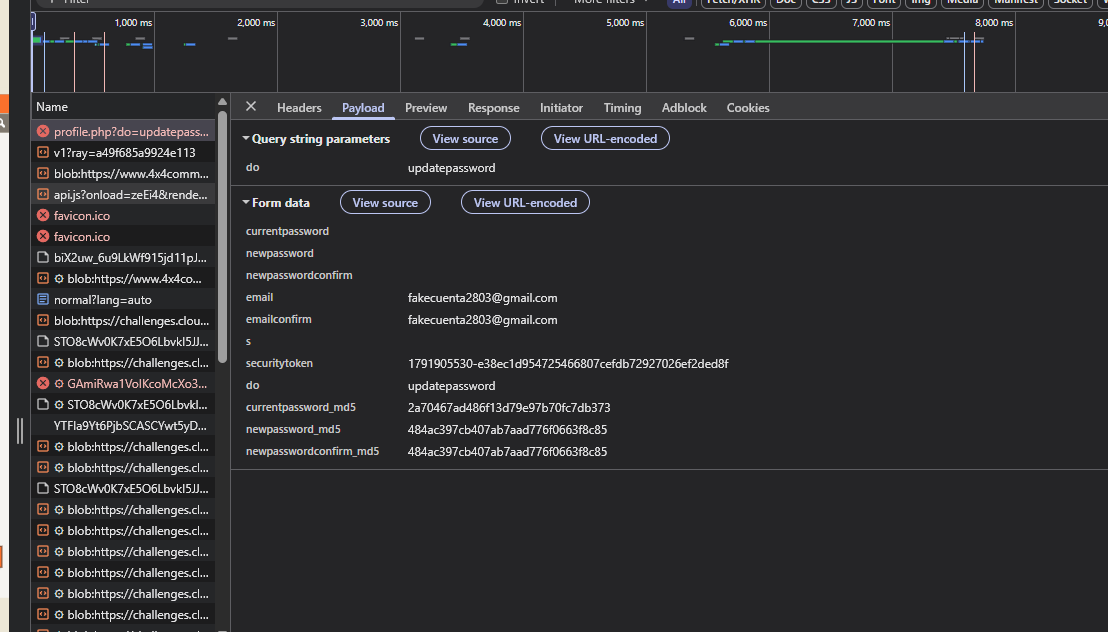
\includegraphics[width=0.85\textwidth]{actividades/cambio_password_payload_md5.png}
    \caption{\textit{Payload} del formulario de cambio de contraseña: también se envía solo el MD5.}
    \label{fig:cambio-payload}
\end{figure}

Las peticiones de este formulario fueron bloqueadas por Cloudflare en varias ocasiones, por lo que la contraseña definitiva se estableció mediante la opción ``olvidé mi contraseña''. El sitio generó una contraseña aleatoria y la \textbf{envió en texto plano por correo electrónico} (Figura \ref{fig:correo-reset}). Esto implica que el servidor tuvo la contraseña en claro y que cualquiera con acceso al correo puede leerla.

\begin{figure}[H]
    \centering
    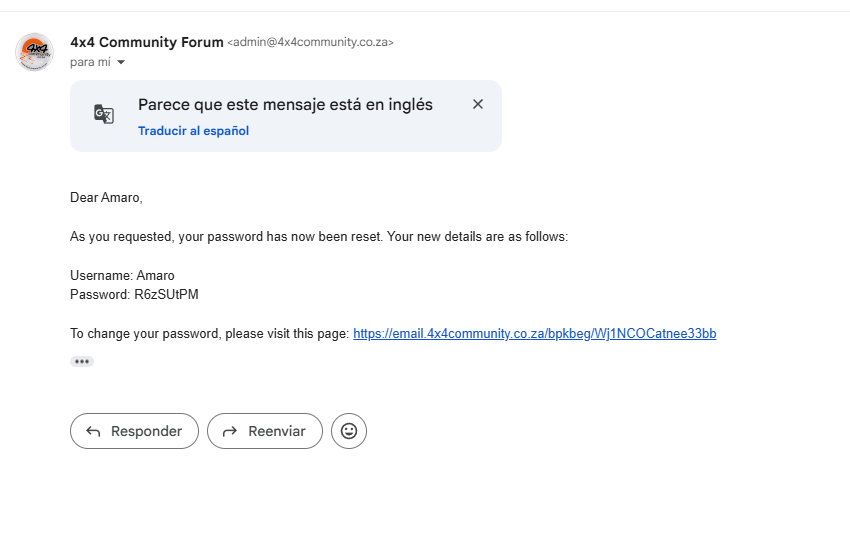
\includegraphics[width=0.75\textwidth]{actividades/correo_reset_password.png}
    \caption{Correo de restablecimiento: el sitio envía la nueva contraseña en texto plano.}
    \label{fig:correo-reset}
\end{figure}

Finalmente, un intento de inicio de sesión con la contraseña del laboratorio es rechazado (Figura \ref{fig:pass-rechazada}), lo que confirma que \texttt{Lab3Cripto2026} y su hash ya no permiten acceder a la cuenta.

\begin{figure}[H]
    \centering
    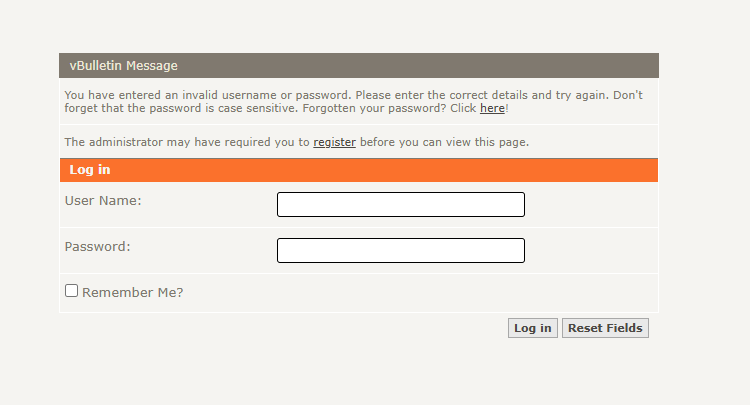
\includegraphics[width=0.75\textwidth]{actividades/login_password_lab_rechazada.png}
    \caption{Inicio de sesión con \texttt{Lab3Cripto2026} rechazado tras el cambio de contraseña.}
    \label{fig:pass-rechazada}
\end{figure}

\subsection{Demuestra 4 conclusiones sobre la seguridad}

\begin{enumerate}
    \item \textbf{El hash en el cliente no protege contra Pass the Hash; solo cambia qué es la ``contraseña''.} Como el servidor acepta el MD5 tal como llega, ese valor pasa a ser la credencial real. Se demostró en la sección 2.5: con una contraseña incorrecta y el hash correcto se inició sesión. La medida evita que la contraseña en texto plano viaje por la red (lo que protege contra su reutilización en otros sitios), pero no impide que quien capture el hash entre a la cuenta.

    \item \textbf{MD5 sin sal es un algoritmo obsoleto para contraseñas.} MD5 es muy rápido de calcular (una GPU actual prueba miles de millones de hashes por segundo) y además está roto frente a colisiones. Al no usar sal, la misma contraseña produce siempre el mismo hash en cualquier sitio vBulletin, por lo que un hash capturado puede buscarse en tablas precalculadas o atacarse por diccionario. Así, el hash no solo permite el PtH, sino que también expone la contraseña original si esta es débil. Lo recomendable es un algoritmo lento y con sal en el servidor, como bcrypt, scrypt o Argon2.

    \item \textbf{El hash es determinista y reutilizable indefinidamente.} El valor enviado fue idéntico en el registro y en cada inicio de sesión, y no incorpora ningún valor aleatorio entregado por el servidor (un \textit{nonce} o desafío). Por eso, un hash interceptado una sola vez sirve para siempre, hasta que el usuario cambie su contraseña. Un esquema de desafío-respuesta (por ejemplo SCRAM) o un protocolo PAKE como OPAQUE evitarían que lo capturado se pueda volver a usar.

    \item \textbf{La seguridad real depende de HTTPS y de capas externas, no del hash.} El único mecanismo que protege el hash en tránsito es TLS; ante un intermediario con un certificado de confianza (como Burp en este laboratorio, o un proxy corporativo o malware en el equipo de la víctima), el hash queda expuesto. Las protecciones observadas, como la verificación anti-bots de Cloudflare y la moderación de cuentas nuevas, no detuvieron el ataque, y el sitio no ofrece autenticación de dos factores. A esto se suma que vBulletin 4.2.5 está fuera de soporte (no recibe actualizaciones de seguridad), que la política de privacidad no menciona cómo se manejan las contraseñas y que, al restablecer la contraseña, el sitio la envía en texto plano por correo electrónico (sección 2.6, Figura \ref{fig:correo-reset}).
\end{enumerate}

\end{document}
